\begin{frame}
\begin{center}
Have you ever had this problem?
\end{center}
\end{frame}

\begin{frame}
\begin{center}
You are writing a data type, such as \lstinline{data Aircraft}
\end{center}
\end{frame}

\begin{frame}
\begin{center}
So you decide that an \lstinline{Aircraft} is the product of
\end{center}
\begin{itemize}
\item \lstinline{Manufacturer}
\item \lstinline{Designation}
\item \lstinline{Registration}
\item \lstinline{Category}
\end{itemize}
\end{frame}

\begin{frame}
\begin{center}
and a \lstinline{Category} is the sum of
\end{center}
\begin{itemize}
\item \lstinline{Aeroplane}
\item \lstinline{Helicopter}
\item \lstinline{Gyroplane}
\item \lstinline{Airship}
\item \ldots
\end{itemize}
\end{frame}

\begin{frame}
\begin{center}
and on the \lstinline{Aeroplane} constructor you have the product of
\end{center}
\begin{itemize}
\item \lstinline{NonEmpty Propulsion}
\item \ldots
\end{itemize}
\end{frame}

\begin{frame}
\begin{center}
and a \lstinline{Propulsion} is the product of
\end{center}
\begin{itemize}
\item \lstinline{Engine}
\item \lstinline{MountPosition}
\end{itemize}
\end{frame}

\begin{frame}
\begin{center}
and an \lstinline{Engine} is the product of
\end{center}
\begin{itemize}
\item \lstinline{Manufacturer}
\item \lstinline{Designation}
\item \lstinline{EngineType}
\end{itemize}
\end{frame}

\begin{frame}
\begin{center}
and an \lstinline{EngineType} is the sum of
\end{center}
\begin{itemize}
\item \lstinline{ICE}
\item \lstinline{Jet}
\item \lstinline{Electric}
\item \lstinline{Rocket}
\end{itemize}
\end{frame}

\begin{frame}
\begin{center}
and an \lstinline{ICE} is the product of
\end{center}
\begin{itemize}
\item \lstinline{AirInduction}
\item \lstinline{FuelInduction}
\item \lstinline{Ignition}
\item \lstinline{ICEType}
\end{itemize}
\end{frame}

\begin{frame}
\begin{center}
and etc etc
\end{center}
\end{frame}

\begin{frame}
\begin{center}
You write all your code in terms of this \lstinline{Aircraft} data type
\end{center}
\end{frame}

\begin{frame}
\begin{center}
Then you create a database schema and store aircraft in it
\end{center}
\end{frame}

\begin{frame}
\begin{center}
\ldots and then \ldots
\end{center}
\end{frame}

\begin{frame}
\begin{center}
Project Manager: ``can we just add an image to internal combustion engines?''
\end{center}
\end{frame}

\begin{frame}[fragile]
\frametitle{oh no}
\begin{center}
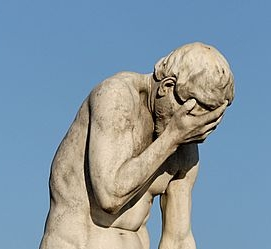
\includegraphics[height=0.24\textheight]{image/ohno.jpg}
\end{center}
\end{frame}

\begin{frame}
\begin{center}
Your data type tree needs to grow
\end{center}
\end{frame}

\begin{frame}
\begin{center}
Trees That Grow is an approach to this extensibility
\end{center}
\end{frame}
